\documentclass[10pt,a4paper, DIV9]{scrartcl}
\usepackage[ngerman]{babel}
\usepackage[applemac]{inputenc} % Diese Umgebung l�sst Umlaute �ber Tastatur zu!
\usepackage[pdftex]{graphicx}
\usepackage[T1]{fontenc}
\usepackage{ae}
\usepackage{amsmath}
\usepackage{amssymb}

\parindent = 0.0in

\title{Eine Drehung der Einheits-Hyperbel $\mathbf{x^2 - y^2 = 1}$ und Hyperbelfunktionen}
\author{Holger Horn}
%***********************************************Seite 1************************************************
\begin{document}
\maketitle
%\sffamily 
%\upshape


Aus der allgemeinen Gleichung einer Hyperbel $ \frac {x^2} {a^2}- \frac {y^2} {b^2}=1 $, bei der die Hauptscheitel $ (\pm a | 0) $ sind und die Asymptoten durch $ (\pm a| \pm b) $ gehen, erh�lt man f�r $ a = b = 1 $ die "`Einheits"'-Hyperbel:
\vspace{1cm}
\begin{center}
\includegraphics[viewport= 145 484 380 716]{Bilder/einhhyp.pdf}
\end{center}
\vspace{1cm}
 Durch Drehung der Asymptoten und der Hyperbel um $O$ um 45� erh�lt man eine Hyperbel, wie sie aus der Analysis gel�ufig ist. Gesucht ist ihre Gleichung (vielleicht $ y = \frac {1}{x} $ ?).
%***********************************************Seite 2************************************************
\section{"`Drehgleichungen"' f�r Drehung um $O(0|0)$ um 45�}

\noindent
\begin{minipage}{0.35\linewidth}
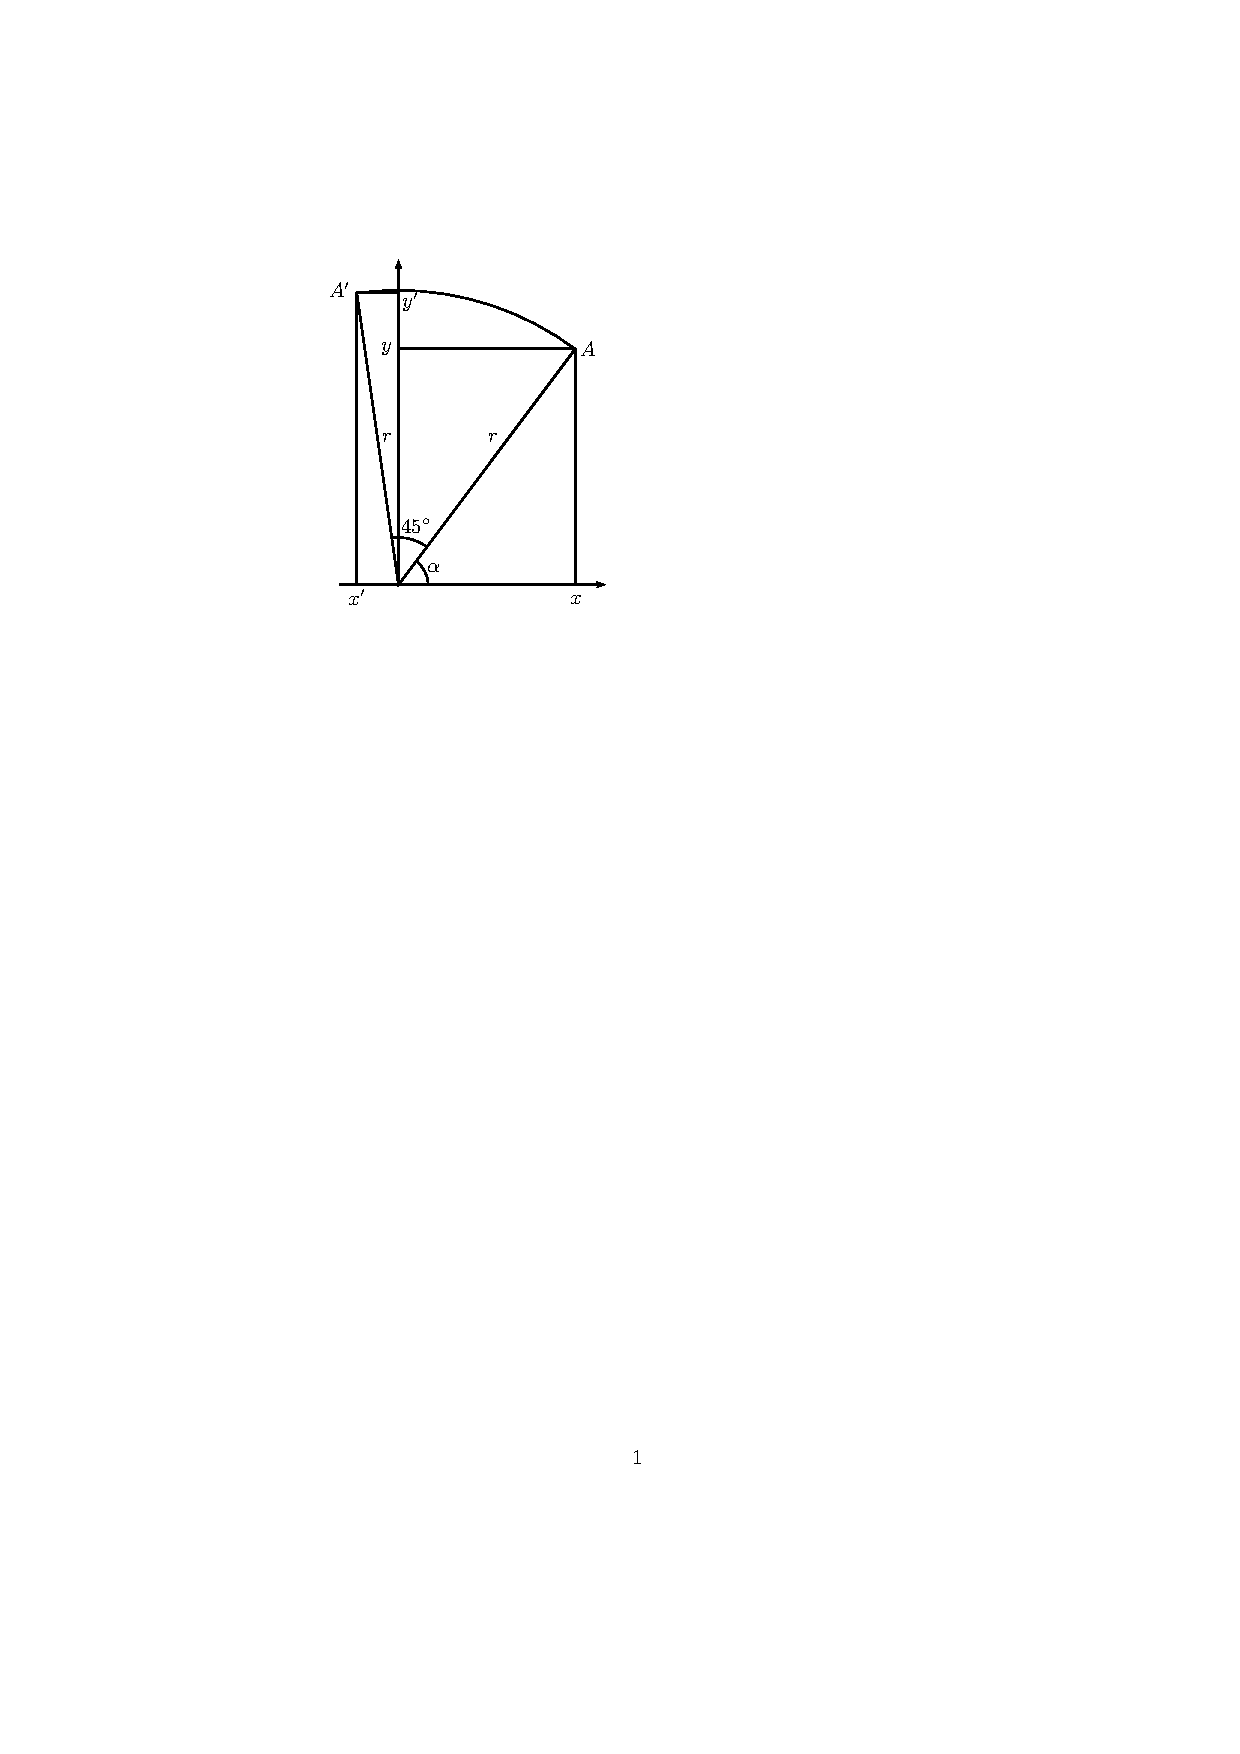
\includegraphics[viewport= 157 550 290 719, clip, width=\linewidth]{Bilder/45rota.pdf}
\end{minipage}
\begin{minipage}{0.65\linewidth}
Aus dem Bild, in dem $A$ um $O$ um 45� gedreht wurde, liest man ab:
$$\sin {\alpha} = \frac{y}{r}; \quad \cos {\alpha} = \frac{x}{r} $$
$$\sin (45^{\circ}+\alpha) = \frac{y'}{r}; \quad \cos (45^{\circ}+\alpha) = \frac{x'}{r}$$
Mit den Additionstheoremen der Winkelfunktionen und $ \sin{45^{\circ}}=\cos{45^{\circ}}=\frac{1}{\sqrt{2}}$ erh�lt man:
$$\frac{y'}{r}=\frac{1}{\sqrt{2}}\cos{\alpha}+\frac{1}{\sqrt{2}}\sin{\alpha}=\frac{1}{\sqrt{2}}(\cos{\alpha}+\sin{\alpha})$$
$$\frac{x'}{r}=\frac{1}{\sqrt{2}}\cos{\alpha}-\frac{1}{\sqrt{2}}\sin{\alpha}=\frac{1}{\sqrt{2}}
(\cos{\alpha} - \sin{\alpha})$$
Durch Multiplikation mit r ergeben sich die "`Drehgleichungen"':
$$\fbox{$x'=\frac{1}{\sqrt{2}}(x-y)\quad \wedge \quad y'=\frac{1}{\sqrt{2}}(x+y)$}$$
\end{minipage}

\section{Drehung der Einheitshyperbel}

Hyperbelgleichung: $x^2-y^2=1\Longrightarrow y=\pm \sqrt{x^2-1}$, betrachte zun�chst die obere H�lfte des Schaubildes: "`+"' und setze in die addierten und subtrahierten Drehgleichungen ein:
$$y'+x' = {\frac{2}{\sqrt{2}}} x; \quad y'-x' = \frac{2}{\sqrt{2}}\sqrt{{x^2}-1}$$
Durch Quadrieren und ineinander Einsetzen erh�lt man:
\begin{eqnarray}\nonumber y'^2-2x'y'+x'^2 & = & 2x^2 - 2\\ \nonumber & = & y'^2+2x'y'+x'^2-2
\end{eqnarray} 
Somit $$-4x'y'= -2 \Longrightarrow 
\fbox{$y' = \frac{1}{2x'}$}
$$
F�r die untere H�lfte des Schaubildes der Einheitshyperbel ("` -- "') ergeben sich dieselben Gleichungen wie oben, nur sind x' und y' vertauscht, was am Endergebnis nichts �ndert.


Die Hyperbel mit der Gleichung $y = \frac{1}{2}\frac{1}{x}$ entsteht aus der Hyperbel mit $y = \frac{1}{x}$ durch "`Stauchung"' in y-Richtung mit dem Faktor $\frac{1}{2}$; da die Hyperbel symmetrisch zur ersten Winkelhalbierenden ist, ist dies gleichzeitig eine Stauchung in x-Richtung mit demselben Faktor! (Eine erstaunliche Eigenschaft dieser Hyperbel! - aller Hyperbeln?)
[Forme in $2xy=1$ um und vertausche x, y! F�r welche weiteren Hyperbeln gilt also diese sch�ne Eigenschaft?]

[Betrachte die Hyperbel mit der Gleichung $\frac{x^2}{a^2}-\frac{y^2}{b^2}=1$ und drehe so, dass die Asymptote durch $(a|b)$ auf die y-Achse abgebildet wird. Allgemein dreht man um $O(0|0)$ um den Winkel $\varphi$ durch:
$$\fbox{$ \bar{x}= x \cos \varphi - y \sin \varphi \quad\wedge\quad  \bar{y}= x \sin \varphi + y\cos \varphi $}$$
(F�r $ \varphi = 45^{\circ} $ ergeben sich die oben verwendeten Gleichungen.)

Nach der Drehung entsteht eine Hyperbel mit einer schr�gen Asymptote; solche Funktionen haben wir in den gebrochen-rationalen Funktionen gefunden, deren Z�hlergrad um eins gr��er als der Nennergrad ist.]
%***********************************************Seite 3************************************************
\section{Hyperbelfunktionen und ihre Beziehung zur Einheitshyperbel}
\noindent
Die Hyperbelfunktionen haben gewisse Analogien zu den Winkelfunktionen (vgl. die Abbildung unten links mit der Definition der Winkelfunktionen im Einheitskreis). Sie sind folgenderma�en definiert:
\begin{eqnarray*} %"*" hat zur Folge, dass Glen. nicht nummeriert werden
\sinh x &=& \frac{e^{x} - e^{-x}}{2} \\ \cosh x &=& \frac{e^{x} + e^{-x}}{2} \quad \text{(Kettenlinie)} \\� \tanh x&=& \frac{\sinh x}{\cosh x} = \frac{e^{x} - e^{-x}}{e^{x} + e^{-x}} = \frac{e^{2x}-1}{e^{2x}+1}
\end{eqnarray*}
Dem trigonometrischen Pythagoras entspricht: $\quad \cosh^{2}x -\sinh^{2} x = 1$.
Damit ergibt sich ein Bezug zur Einheitshyperbel: Setzt man $x = \cosh t $ und $ y = \sinh t$, so hat man eine Parameterdarstellung der Hyperbel, wobei sich  uns die Bedeutung des Parameters noch erschlie�en wird. Betrachte dazu das Bild; ferner l�sst sich aus dem Bild mit dem 2. Strahlensatz entnehmen: 
$$\frac{\tanh t}{1}= \frac{\sinh t}{\cosh t}$$


%\vspace{0.5cm}
\noindent
\begin{minipage}{0.35\linewidth}
\includegraphics[viewport= 135 520 264 714, clip]{Bilder/defhypfkt.pdf}
\begin{center}
Man beachte die 1,5-fache\\L\"angeneinheit in y-Richtung!
\end{center}
\end{minipage}
\begin{minipage}{0.13\linewidth}
$$ $$
\end{minipage}
\begin{minipage}{0.52\linewidth}
	\begin{center}
		\includegraphics[viewport= 50 490 280 730, clip, width=\linewidth]{Bilder/hypfkt.pdf}
		
		Die Graphen der Hyperbelfunktionen
	\end{center}
	\label{fig:hypfkt}
\end{minipage}
%***********************************************Seite 4************************************************
\newpage
\begin{center}
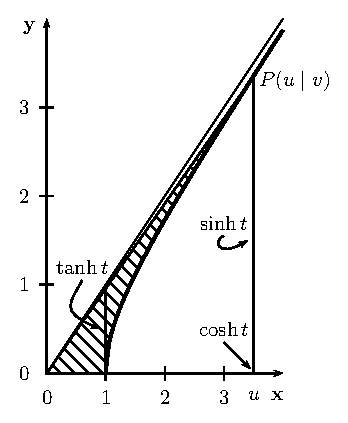
\includegraphics[viewport= 134 527 285 714] {Bilder/bezhypfkt}
\end{center}

Inhalt A der schraffierten Fl�che in obigem Bild.
Die Fl�che wird durch die Gerade OP (Steigung ist tanh t), die x-Achse und die Einheitshyperbel begrenzt.
\begin{eqnarray*}
A &=& A_{\triangle}- \int_{1}^{u}\sqrt{x^{2}-1}dx\\
&=& \frac{1}{2}u\sqrt{u^{2}-1}- \left [\frac{x}{2}\sqrt{x^{2}-1}-\frac{1}{2}\ln\left |x+\sqrt{x^{2}-1}\right | \right ]_{1}^{u} \qquad \text{(vgl. Formelsammlung)}
\end{eqnarray*}
Also gilt
$$\fbox{$A = \frac{1}{2}\ln\left (u + \sqrt{u^{2}-1}\right ) \qquad (u>0)$}$$

Nun l�sst sich der Parameter t deuten: 
\begin{eqnarray}\nonumber
u = \cosh t = \frac{e^{t}+e^{-t}}{2} &\Longrightarrow& 2u = e^{t}+e^{-t} \quad | \cdot e^{t}\\
\nonumber\Longrightarrow  2ue^{t} = e^{2t}+1 &\Longrightarrow& e^{2t}- 2ue^{t}+1 = 0\\
\nonumber\Longrightarrow e^{t}= u \pm \sqrt{u^{2}-1} &\Longrightarrow& t = ln \left (u \pm \sqrt{u^{2}-1}\right )
\end{eqnarray}
Ergebnis: Der Parameter t ist das Doppelte der zugeh�rigen schraffierten Fl�che!

�berlege, wie mit $\pm$ im Ergebnis f�r t umzugehen ist; welches Zeichen gilt?

[�bung: Werte das Integral ohne Benutzung der Formelsammlung aus!]



\end{document}